%Template and commentary by Michael Rouleau: https://github.com/mikerouleau/ME4842.git
%Text primarily from Dr. Stutts' Systems Laboratory Manual /ref{Stutts}
%Last Updated: Feb 13, 2019

%----This template includes equation captions and numbering BELOW the equation, as required by Blaine Allen----%

\documentclass[11pt,letter]{report}
\usepackage[margin=1in]{geometry} %make margins 1"
\usepackage[justification=centering, format=plain,
font=it, margin=1in]{caption} %all captions centered and made italics by default
\usepackage{amsmath, amssymb} %advanced math extensions
\usepackage{graphicx} %enhanced graphics handling/management
\usepackage{float} %create floating containers
\usepackage{aliascnt} %alias counters as needed

%for the commentary section only
\usepackage{hyperref}
\usepackage{xcolor}
\definecolor{lightgray}{gray}{0.97}
\usepackage{listings} %For code in appendix
\lstset{language = [LaTeX]TeX,     breaklines=true,
	    numbers=left, backgroundcolor=\color{lightgray}}



%make equations floating objects and alias counter - needed for formatting requirements
\newaliascnt{eqfloat}{equation} %make the counter alias eqfloat
\newfloat{eqfloat}{!htb}{eqflts} %make the float container for equations
\floatname{eqfloat}{Equation} %change name so captions read "Equation" X:
        
%nontraditional usage of author to meet formatting requirements
\title{\Huge{Systems Lab \LaTeX\ Template Commentary}}
\author{Section \#, Group \#: \\
  Group Member 1 \quad Group Member 2 \quad Group Member 3 \quad Group Member 4 \\ GTA: Blaine Allen \\\\ Prepared By: \\ Michael Rouleau\thanks{The original template stems from formatting guidelines in the course manual\cite{Stutts}.}}
\date{\today}

\begin{document}
\maketitle

\chapter{Using \LaTeX{}} \label{chap:usinglatex}
	\section{About \LaTeX{}}
	\LaTeX{}, pronounced "Lah-tech" or "Lay-tech" \cite{Lamport}, is an advanced document preparation system frequently used in the scientific world and academia. Instead of organizing a document visually like a WYSIWYG (what you see is what you get) package (e.g. Microsoft Word), \LaTeX{} has a logical structure that focuses on content rather than formatting decisions. This means that if you decide that all of your fractions of the form $\tfrac{x}{y}$ require a little extra size, as in $\dfrac{x}{y}$, the entire document can be reformatted with these requirements in just a line or two of code. Similarly, it is possible to compile a list of sources that were used during research, then automatically list and number only those which were cited in the manuscript. Did I mention your citations auto-update too? Complex mathematical notations are just a few keystrokes away (instead of digging in a symbol library). For long scientific documents, \LaTeX{} is the cat's meow.
	
	\section{Installation} \label{sect:install}
	To start editing a \LaTeX{} document on a Missouri S\&T Computer, simply log on to AppsAnywhere and start the program "Texmaker."
	
	For personal computers, Texmaker is freely available from \url{http://www.xm1math.net/texmaker/} and its dependency, MiKTeX, is available from \url{https://miktex.org/}. Installing MiKTex before Texmaker is recommended. Detailed installation instructions are available from each package's respective website. It is also possible to run a portable installation of the above from a USB drive.
	
	\section{Basics} \label{sect:basics}
		\subsection{Syntax}
		\LaTeX{} code is typed into a plain-text file called an "input" or "source" file that contains markup which tells the compiler how to display content. In general, the following reserved characters demarcate normal text and commands or other special functions:

		\begin{center}		
		\# \$ \% \^{} \& \_ \{ \} \~{} \textbackslash{}.
		\end{center}

		It is still possible to use these symbols, but they typically require a backslash prefix.

		\begin{center}		
		\verb|\# \$ \% \^{} \& \_ \{ \} \~{} \textbackslash{}|.
		\end{center}

		Commands also usually require a \textbackslash{} prefix. For example,
		\verb|\textbf{Bold}| turns text \textbf{Bold}. Commands can also be nested, as \verb|\textbf{\textit{Italics and Bold!}}| turns text both \textit{\textbf{Italics and Bold!}}
		
		Backslashes can also signal an environment. Environments act similar to commands but are usually applied to multiple lines or more complex operations. For example,
		

\begin{lstlisting}[numbers=left,xleftmargin=5mm]
\begin{figure}
\includegraphics{joeminer}
\end{figure}
\end{lstlisting}


		would insert a figure named "joeminer" from the directory my file is saved in.
		
		Comments can be added with the \% symbol. The compiler will ignore the remainder of the current line and any whitespace at the beginning of the following line. This can be useful for adding notes that should not be included in the final version.
	\section{Structure}
		The minimum structure of a \LaTeX{} document is best illustrated with the following "Hello World" example. Feel free to follow along in Texmaker.
		

\begin{lstlisting}[numbers=left,xleftmargin=5mm]
\documentclass{article}
\begin{document}
Hello World!
\end{document}
\end{lstlisting}

	
		Breaking down each line, we have an initial declaration of what class the document is - this sets basic definitions for formatting. In this example, we're using the article class, which is a common starting point.
		
		The second line is where the document officially starts. This is where the environment called "document" begins - all of your content will go between the \verb|\begin{document}| and \verb|\end{document}| tags. Everything before this point is traditionally called the "Preamble." If you are including any external packages or redefining commands, do it in the Preamble.
		
		Our content, of course, only consists of "Hello World!". This is where your entire report, book, manuscript, etc. would go.
		
		\verb|\end{document}| ends the document environment. Anything after this line is ignored.
		
		To compile your first \LaTeX{} document, save your file (without spaces!) and click the (left) "Run" arrow in the top tool bar of Texmaker. Your new document should appear on the right side of the window. For simple documents, only one compilation is necessary. For complex documents (especially those with intricate references), multiple compilation steps may be required.s
		
	\section{Organization} \label{sect:org}
		\LaTeX{} commands for breaking up documents are intuitive. For example, \verb|\chapter{Silver}| starts a new chapter named "Silver" and \verb|section{Gold}| starts a new section called "Gold." It is left as an exercise to discover what \verb|\subsection{text}| and \verb|\subsubsection{text}| do.
		
		For each of these commands, a number or other counter is inserted by default. To create an unnumbered heading, the "starred" version may be used. For example, a unnumbered section heading would use \verb|\section*{text}|. To manually adjust the count, the command \verb|\setcounter{countername}{#}| is used.
		
		Paragraphs are created by placing a blank line before the start of the next paragraph. Any additional blanks lines are ignored.

%todo floats, positioning, [!htbpH]

\chapter{The Template} \label{chap:template}
	\section{Preamble} \label{sect:preamble}
		With these basics under our belt, we can decode the Lab Template. Let's look at the preamble together.

	\begin{lstlisting}[numbers=left,xleftmargin=5mm]
%Template and commentary by Michael Rouleau: https://github.com/mikerouleau/ME4842.git
%Text primarily from Dr. Stutts' Systems Laboratory Manual /ref{Stutts}
%Last Updated: Feb 15, 2019

%----This template includes equation captions and numbering BELOW the equation----%

\documentclass[11pt,letter]{report}
\usepackage[margin=1in]{geometry}
\usepackage[justification=centering, format=plain, font=it, margin=1in]{caption}
\usepackage{amsmath, amssymb}
\usepackage{graphicx}
\usepackage{float}
\usepackage{aliascnt}
\newaliascnt{eqfloat}{equation}
\newfloat{eqfloat}{!htb}{eqflts}
\floatname{eqfloat}{Equation}

%nontraditional usage of author to meet formatting requirements
\title{\Huge{}A Systems Lab Memo}}
\author{Section \#, Group \#: \\
Group Member 1 \quad Group Member 2 \quad Group Member 3 \quad Group Member 4 \\ GTA: Blaine Allen \\\\ Prepared By: \\ Michael Rouleau\thanks{Nearly all of this information is from the course manual\cite{Stutts}; I simply formatted it.}}
\date{\today}
	\end{lstlisting}
	
		Lines 1-6 contain notes to whoever is reading the code. It is good practice to comment your name and date as a bare minimum.
		
		Line 7 defines the document class, just like we did in Section \ref{sect:org}. The only difference is that now we have declared a couple of options: paper size and normal text font size. While these may be set by a class, using an option overrides the default settings.
		
		Lines 8-13 all include various external packages. The geometry package allows us to define margins of 1". Caption changes the default font settings for our figure and equation captions. Amsmath and amssymb (note we are being sneaky and including two packages at once) provide some fancy commands and environments for math. We'll primarily be using the equation environment. Graphicx allows us to insert figures with \verb|\includegraphics{imagefile}|. Finally, the float and aliascnt packages are used for some fancy manipulation of equations in order to meet the formatting requirements.
		
		Speaking of formatting gymnastics, lines 16-18 is where the most complex of it takes place. In line 16, we define a new alias count called "eqfloat." This alias essentially acts as another name for the counter it follows, "equation." This means if eqfloat is indexed, equation will also be indexed and vice versa. Line 17 takes eqfloat and defines a float container also named "eqfloat". [!htb] defines our preferred placements, and "eqflts" is the name it appears in the log file under. The float implicitly inherits the counter alias from line 16 - each eqnfloat environment is counted with the equation counter. Line 18 changes the name of the float to be "Equation." By doing this, the \verb|\caption{text}| command will read Equation: \#, instead of eqfloat: \#.
		
		Finally lines 21-24 pertain to the title page. This section is fairly self-explanatory. However, you'll note the use of \verb|\quad| and \verb|\\| within the author command. \verb|\quad| helps with the spacing of authors. Even if you don't have 4 group members, \verb|\quad| will likely still work to distribute them in an aesthetic manner. \verb|\\| on the other hand, serves as a complex macro that introduces a line break in this context. Limit the use of \verb|\\| unless necessary.

	\section{Body} \label{sect:body struct}
		After the Preamble, \verb|\begin{document}| begins the document environment. Immediately after, we use the \verb|\maketitle| command to generate the title page of our document before diving into our content. Since the body usage is repetitive, let's break the template up further into the different environments and their usage.
		
		\subsection{Sections} \label{subsect: sections}
			Just as described in Section \ref{sect:org}, the command \verb|\section*{Section Title}| defines the beginning of a new section. The "starred" version of this command removes the section number from showing up on your final report. For each new section, simply add the \verb|\section| command and type the name of the new section in curly brackets following it.
			
		\subsection{Tables} \label{subsect:table}
			Tables are perhaps the most difficult format of data to insert in \LaTeX{}. Fortunately, we can logically break down each line again.
			
			\begin{lstlisting}[numbers=left,xleftmargin=5mm]
\begin{table}[!htb]
	\caption{Annual Per Capita Consumption of Mozzarella Cheese and Civil Engineering Doctorates Awarded \cite{Vigen}}
	\label{table:Civil Cheese}
	\centering
	\begin{tabular}{|c|c|c|}
		\hline
		\textbf{Year} & 
			\textbf{\begin{tabular}[c]{@{}c@{}}
			Civil Engineering\\ 
			Doctorates\end{tabular}} &
				\textbf{\begin{tabular}[c]{@{}c@{}}
				Mozzarella\\
				Cheese Consumption
				\end{tabular}} \\ \hline
		2000  & 480  & 9.3     \\ \hline
		2001  & 501  & 9.7     \\ \hline
		2002  & 540  & 9.7     \\ \hline
		2003  & 552  & 9.7     \\ \hline
		2004  & 547  & 9.9     \\ \hline
	\end{tabular}
\end{table}
			\end{lstlisting}

			At this point, you should be able to guess what line 1 does - it marks the beginning of a table environment. Since tables are floating environments, the \verb|[!htb]| tag tells the compiler where to place the table, in order of preference. Refer to Section \ref{sect:org} for more options. Essentially, H turns a floating object into a non-floating object  Line 2 adds a caption above the table, complete with a citation - we'll get to those later, in Section \ref{sect:ref}.
			Line 3 adds a reference label to the table. Again, we'll cover what this means in Section \ref{sect:ref}. Line 4 tells the compiler to center the current paragraph, or in this case, table.
			
			Line 5 is where the fun begins. First, we start a tabular environment within the table environment and define the number of columns (3) using \{$|$c$|$c$|$c$|$\}. Note that c does not refer to "column." Instead, c refers to centered - the formatting for each column's data. Other popular options are "l" for left and "r" for right alignment. Line 6 inserts a horizontal line that is the width of our table. 
			
			Lines 7-14 start off easy - the first cell in our table, moving left to right from the top is Year, in bold text. \& signifies the end of the cell, and we move into our second cell on line 8. Picking this cell apart, we have a \verb|\textbf{}| command again - so this cell is also in bold text. Within it, another tabular environment starts. This second environment allows us to create subcells within the cell - one for "Civil Engineering" and the other for "Doctorates." Unfortunately, the standard tabular package does not support \verb|\newline| or \verb|\linebreak|, so this is the best native workaround I am aware of. In declaring this new tabular environment, we use \verb|[c]{@{}c@{}}| - different from the first time. [c] in this case is our vertical alignment - again, centered. Other options include t for top and b for bottom. Our horizontal parameters are taken care of within the curly brackets. \verb|@{}| overrides any horizontal padding on each side of these subcells, and c is again horizontal alignment for the single column of subcells. The contents of each subcell is on lines 9 and 10, with a \verb|\\| to demarcate the end of a row. With an \$ to move us into the next cell, the same process is repeated for our final title cell. After all three cells in the top row are full, \verb|\\ \hline| is used to mark the end of the row and insert a horizontal line.

			Armed with this information, lines 15-21 should be easy to figure out.
			
		\subsection{Figures} \label{subsect:fig}
			Figure insertion is a comparatively trivial process. Simply by looking at the code below, most of it should be easily understood.
			
			\begin{lstlisting}[numbers=left,xleftmargin=5mm]
\begin{figure}[!htb]
\label{fig:Cat Lord}
\centering
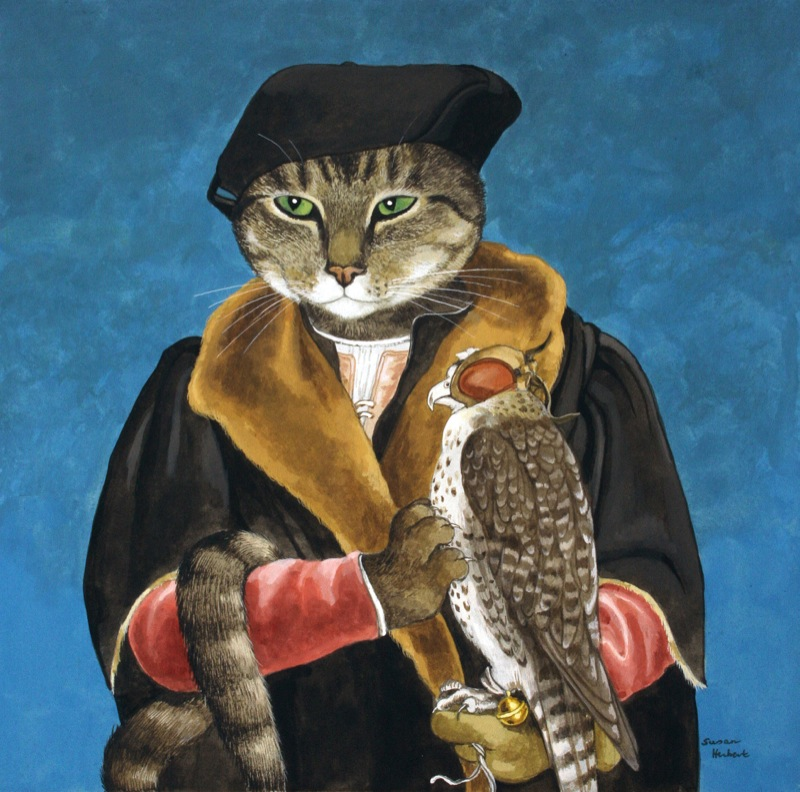
\includegraphics[scale=0.4]{cat-painting}
\caption{Robert Cheseman (Holbein)\cite{Herbert}}
\end{figure}
			\end{lstlisting}
	
			As expected, \verb|\begin{figure}[!htb]| starts a figure environment. Figures are floating environments, so we provide them with placement preferences. As we've seen before, \verb|\label{key}| defines a label and \verb|\centering| centers the figure.
			
			The includegraphics command takes the form of  \verb|\includegraphics[options]{imagefile}|, where options are things like height, width, and scale can be set. Our feline friend is a bit on the large side, we've scaled him down to 40\%. Purrfect! The imagefile field takes the filepath of the image as input - no need to add an extension, the compiler will search for all supported formats. Each time the compiler runs, it searches for the figure file and re-inserts it. This means that if you need to swap out a figure, simply upload the new figure to the same directory and rename the new and old files appropriately. Next time the compiler is run, the new figure will appear.
			
			Finally, we have a caption, complete with citation. For more information on citations, refer to Section \ref{sect:ref}.
		
		\subsection{Lists} \label{subsect:lists}
			A convenient way to format a procedure section of a lab report is as a list. For most situations, a numbered list will suffice, taking the form of
			
			\begin{lstlisting}[numbers=left,xleftmargin=5mm]
\begin{enumerate}
\item First item
\item Second item
\item Third item
\end{enumerate}
			\end{lstlisting}
			
			Here, we begin an enumerate environment and indicate the start of each line item as an \verb|\item|. The same process works for an unordered list using the itemize environment. The syntax is identical.
			
			For more complex lists, it is possible to nest lists. For example, 
			
			\begin{lstlisting}[numbers=left,xleftmargin=5mm]
\begin{enumerate}
\item First item
\item \begin{enumerate}
	\item First subitem
	\item Second subitem
	\end{enumerate}
\item \begin{itemize}
	\item First subitem
	\item Second subitem
	\end{itemize}
\end{enumerate}
			\end{lstlisting}
			
			generates the following list:
			
			\begin{enumerate}
				\item First item
				\item \begin{enumerate}
					\item First subitem
					\item Second subitem
				\end{enumerate}
				\item \begin{itemize}
					\item First subitem
					\item Second subitem
				\end{itemize}
			\end{enumerate}
			
		\subsection{Equations} \label{subsect:eqn}
			Equations are one of the significant strengths of any \LaTeX{} package. Te 
			
	\section{References} \label{sect:ref}
		%TODO and bibliography

\section*{Abstract}
The Abstract should be approximately 100-150 words in length. This may be a very strict limit in some cases. For ME4842, the limit will be somewhat flexible. This should include what the objective of the experiment was and its importance, any theory the experiment is based on, major findings and trends found in your results, and a brief summary of your interpretations and conclusions. You should not reference anything in the abstract; this section should be completely independent from the rest of the report.

\section*{Procedure}
Here, you will briefly explain what steps you followed in conducting the experiment. The procedure should state what is not covered in the lab manual and what decisions you made in order to accomplish the experiment. It may be handy to organize this section as a list.

\section*{Results}
Here, you will explain the data you took, and any calculations that you made. This section should be the longest in the report. Many results can be displayed using objects similar to Table~\ref{table:Civil Cheese} and Figure~\ref{fig:Cat Lord}, displayed below.

%Tools such as those at https://www.tablesgenerator.com/ may be useful for creating tables quickly.

%example table formatting
\begin{table}[!htb]
\caption{Annual Per Capita Consumption of Mozzarella Cheese\\ and Civil Engineering Doctorates Awarded \cite{Vigen}} %\cite{name} refers to a specific bibliography entry.
\label{table:Civil Cheese} %use this label to refer to the object elsewhere, as shown in the previous paragraph.
\centering
\begin{tabular}{|c|c|c|}
\hline
\textbf{Year} & \textbf{\begin{tabular}[c]{@{}c@{}}Civil Engineering\\ Doctorates\end{tabular}} & \textbf{\begin{tabular}[c]{@{}c@{}}Mozzarella\\ Cheese Consumption\end{tabular}} \\ \hline
2000  & 480  & 9.3     \\ \hline
2001  & 501  & 9.7     \\ \hline
2002  & 540  & 9.7     \\ \hline
2003  & 552  & 9.7     \\ \hline
2004  & 547  & 9.9     \\ \hline
2005  & 622  & 10.2    \\ \hline
2006  & 655  & 10.5    \\ \hline
2007  & 701  & 11.0    \\ \hline
2008  & 712  & 10.6    \\ \hline
2009  & 708  & 10.6    \\ \hline
\end{tabular}
\end{table}

%example figure formatting
\begin{figure}[!htb]
\label{fig:Cat Lord}
\centering
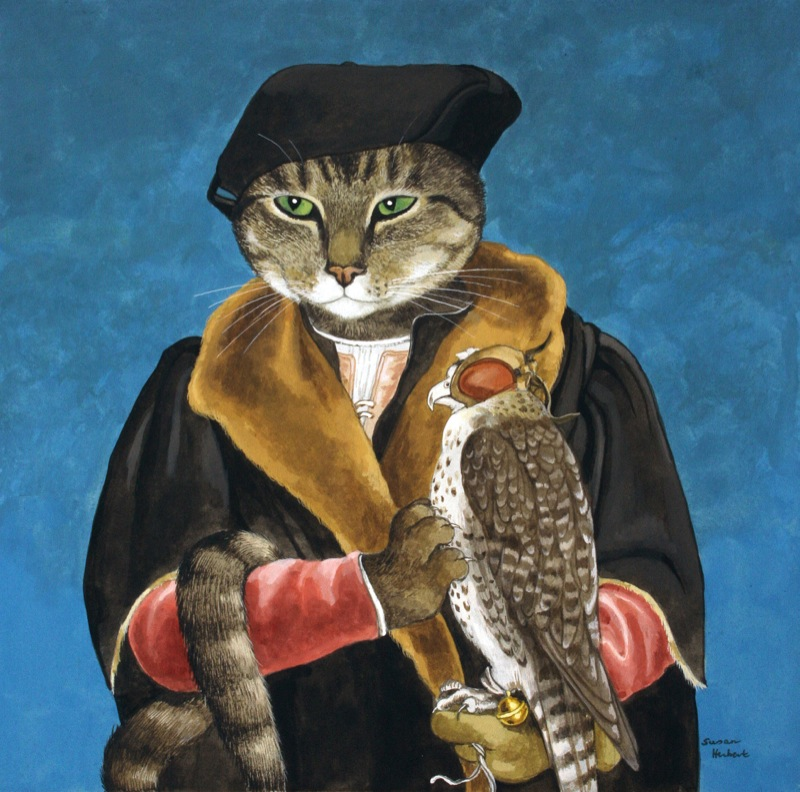
\includegraphics[scale=0.4]{cat-painting}%include full file path unless source file is in the same directory.
\caption{Robert Cheseman (Holbein)\cite{Herbert}}
\end{figure}

\begin{enumerate} %start numbered list
  \item You should be mindful of the number of significant digits you use in your results.
  \item Use consistent units and suitable unit prefixes.
  \item When referring to equations, figures, tables, and appendices in your memo you must always capitalize E in equation F in figure, T in table, and A in appendix.
  \item To reference an equation from the manual don't say "according to Equation 8.25 in the manual". The correct way to do this is: "according to Equation 2 [X]”. Note Equation 2 is an equation in your memo and has its own number and [X] is the citation number in your reference section corresponding to the appropriate source.
  \item Table, figure, and equation titles: Tables get titles on top. Figures and equations get the title on the bottom.
  \item Tables, figures and equations must be part of the written text. That is you should put your table, figure, and equation right below the paragraph where they are first mentioned.
  \item Only include necessary data in tables that are related to the analysis of the experiment.
\end{enumerate}

\section*{Discussion Questions}
In this section, simply answer each question from the lab manual in order. It may be wise to number your responses. Some responses require equations. Equation~\ref{Quadratic} displays the proper formatting; Equation~\ref{eq:Dirac} is a more complex example.

\begin{eqfloat}[!htb]
\begin{equation*}
x=\frac{-b\pm\sqrt{b^2-4ac}}{2a}
\end{equation*}
\caption{The Quadratic Formula}\label{Quadratic}
\end{eqfloat}
	
\begin{eqfloat}
\begin{equation*}
\left (
    \beta mc^2 + c 
       \left ( 
           \sum_{n=1}^3 \alpha_n p_n 
       \right )
\right )
\psi(x,t)
=
i \hbar \dfrac{\partial \psi(x,t) }{\partial t}
\end{equation*}
\caption{The Original Dirac Equation}\label{eq:Dirac}
\end{eqfloat}
%note that the equation numbering auto-increments and the in-line references update accordingly. Tables and figures behave the same way.

\begin{eqfloat}[!htb]
	\begin{equation*}
	x=\frac{-b\pm\sqrt{b^2-4ac}}{2a}
	\end{equation*}
	\caption{The Quadratic Formula}\label{Quatdratic}
\end{eqfloat}

\begin{eqfloat}[!htb]
	\begin{equation*}
	x=\frac{-b\pm\sqrt{b^2-4ac}}{2a}
	\end{equation*}
	\caption{The Quadratic Formula}\label{Quadrattic}
\end{eqfloat}

\section*{Conclusion}
Conclusions should clearly state how well the objective was met, any errors that were part of your data collections or would have affected results, suggestions to improve experimental data collection, and what you might have done better. If you are going to make suggestions for improving the experiment, ensure they are technically sound and would make a significant impact on results.

%A pure LaTeX bibliography 
\begin{thebibliography}{3} %{3} is the number of entries to be added. The maximum value is 99.

\bibitem{Herbert}
  Herbert, S.,\emph{Robert Cheseman (Holbein).}
  Chris Beetles Gallery, London, England, www.chrisbeetles.com/gallery/animals/cats/robert-cheseman-holbein.html. Accessed 8 Nov. 2018.
  
\bibitem{Stutts}
  Stutts, D.S., \emph{Mechanical Engineering Systems Laboratory Manual.}
  Department of Mechanical and Aerospace Engineering, Missouri University of Science and Technology, 3 Oct. 2018. 130-131.
  
\bibitem{Vigen}
  Vigen, T., \emph{15 Insane Things That Correlate With Each Other.}
  Spurious Correlations, tylervigen.com/spurious-correlations. Accessed 8 Nov. 2018.

\bibitem{Lamport}
	Lamport, L., \emph{LATEX: a document preparation system: user's guide and reference manual.} Addison-wesley. 1994.

\bibitem{Gratzer}
	Gratzer, G.A., \emph{Practical LaTeX.} 2014.
\end{thebibliography}

\newpage %force a new page
\section*{Appendix A: Additional Data}
Only thing to put in the appendix is programming codes, program code output, and large raw data tables that are not referenced in any results.

\newpage 
\section*{Appendix B: Usage}
If you run into problems using this template, feel free to contact the author at msr5h7@mst.edu.
\par test

\end{document}